%%%%%%%%%%%%%%%%%%%%%%%%%%%%%%%%%%%%%%%%%
% Programming/Coding Assignment
% LaTeX Template
%
% This template has been downloaded from:
% http://www.latextemplates.com
%
% Original author:
% Ted Pavlic (http://www.tedpavlic.com)
%
% Note:
% The \lipsum[#] commands throughout this template generate dummy text
% to fill the template out. These commands should all be removed when 
% writing assignment content.
%
% This template uses a Perl script as an example snippet of code, most other
% languages are also usable. Configure them in the "CODE INCLUSION 
% CONFIGURATION" section.
%
%%%%%%%%%%%%%%%%%%%%%%%%%%%%%%%%%%%%%%%%%

%----------------------------------------------------------------------------------------
%	PACKAGES AND OTHER DOCUMENT CONFIGURATIONS
%----------------------------------------------------------------------------------------

\documentclass{article}

\usepackage{fancyhdr} % Required for custom headers
\usepackage{lastpage} % Required to determine the last page for the footer
\usepackage{extramarks} % Required for headers and footers
\usepackage[usenames,dvipsnames]{color} % Required for custom colors
\usepackage{graphicx} % Required to insert images
\usepackage{subcaption}
\usepackage{listings} % Required for insertion of code
\usepackage{courier} % Required for the courier font
\usepackage{amsmath}

% Margins
\topmargin=-0.45in
\evensidemargin=0in
\oddsidemargin=0in
\textwidth=6.5in
\textheight=9.0in
\headsep=0.25in

\linespread{1.1} % Line spacing

% Set up the header and footer
\pagestyle{fancy}
\lhead{\hmwkAuthorName} % Top left header
\chead{\hmwkClass\ (\hmwkClassTime): \hmwkTitle} % Top center head
%\rhead{\firstxmark} % Top right header
\lfoot{\lastxmark} % Bottom left footer
\cfoot{} % Bottom center footer
\rfoot{Page\ \thepage\ of\ \protect\pageref{LastPage}} % Bottom right footer
\renewcommand\headrulewidth{0.4pt} % Size of the header rule
\renewcommand\footrulewidth{0.4pt} % Size of the footer rule

\setlength\parindent{0pt} % Removes all indentation from paragraphs

%----------------------------------------------------------------------------------------
%	CODE INCLUSION CONFIGURATION
%----------------------------------------------------------------------------------------

\definecolor{mygreen}{rgb}{0,0.6,0}
\definecolor{mygray}{rgb}{0.5,0.5,0.5}
\definecolor{mymauve}{rgb}{0.58,0,0.82}

\lstset{ %
  backgroundcolor=\color{white},   % choose the background color
  basicstyle=\footnotesize,        % size of fonts used for the code
  breaklines=true,                 % automatic line breaking only at whitespace
  captionpos=b,                    % sets the caption-position to bottom
  commentstyle=\color{mygreen},    % comment style
  escapeinside={\%*}{*)},          % if you want to add LaTeX within your code
  keywordstyle=\color{blue},       % keyword style
  stringstyle=\color{mymauve},     % string literal style
}

%----------------------------------------------------------------------------------------
%	DOCUMENT STRUCTURE COMMANDS
%	Skip this unless you know what you're doing
%----------------------------------------------------------------------------------------

% Header and footer for when a page split occurs within a problem environment
\newcommand{\enterProblemHeader}[1]{
%\nobreak\extramarks{#1}{#1 continued on next page\ldots}\nobreak
%\nobreak\extramarks{#1 (continued)}{#1 continued on next page\ldots}\nobreak
}

% Header and footer for when a page split occurs between problem environments
\newcommand{\exitProblemHeader}[1]{
%\nobreak\extramarks{#1 (continued)}{#1 continued on next page\ldots}\nobreak
%\nobreak\extramarks{#1}{}\nobreak
}

\setcounter{secnumdepth}{0} % Removes default section numbers
\newcounter{homeworkProblemCounter} % Creates a counter to keep track of the number of problems
\setcounter{homeworkProblemCounter}{0}

\newcommand{\homeworkProblemName}{}
\newenvironment{homeworkProblem}[1][Problem \arabic{homeworkProblemCounter}]{ % Makes a new environment called homeworkProblem which takes 1 argument (custom name) but the default is "Problem #"
\stepcounter{homeworkProblemCounter} % Increase counter for number of problems
\renewcommand{\homeworkProblemName}{#1} % Assign \homeworkProblemName the name of the problem
\section{\homeworkProblemName} % Make a section in the document with the custom problem count
\enterProblemHeader{\homeworkProblemName} % Header and footer within the environment
}{
\exitProblemHeader{\homeworkProblemName} % Header and footer after the environment
}

\newcommand{\problemAnswer}[1]{ % Defines the problem answer command with the content as the only argument
\noindent\framebox[\columnwidth][c]{\begin{minipage}{0.98\columnwidth}#1\end{minipage}} % Makes the box around the problem answer and puts the content inside
}

\newcommand{\homeworkSectionName}{}
\newenvironment{homeworkSection}[1]{ % New environment for sections within homework problems, takes 1 argument - the name of the section
\renewcommand{\homeworkSectionName}{#1} % Assign \homeworkSectionName to the name of the section from the environment argument
\subsection{\homeworkSectionName} % Make a subsection with the custom name of the subsection
\enterProblemHeader{\homeworkProblemName\ [\homeworkSectionName]} % Header and footer within the environment
}{
\enterProblemHeader{\homeworkProblemName} % Header and footer after the environment
}

%----------------------------------------------------------------------------------------
%	NAME AND CLASS SECTION
%----------------------------------------------------------------------------------------

\newcommand{\hmwkTitle}{Assignment 1} % Assignment title
\newcommand{\hmwkDueDate}{Monday, January 29, 2018} % Due date
\newcommand{\hmwkClass}{CSC411} % Course/class
\newcommand{\hmwkClassTime}{LEC 5101} % Class/lecture time
\newcommand{\hmwkAuthorName}{Zhongtian Ouyang} % Your name

%----------------------------------------------------------------------------------------
%	TITLE PAGE
%----------------------------------------------------------------------------------------

\title{
\vspace{2in}
\textmd{\textbf{\hmwkClass:\ \hmwkTitle}}\\
\normalsize\vspace{0.1in}\small{Due\ on\ \hmwkDueDate}\\
\vspace{0.1in}
\vspace{3in}
}

\author{\textbf{\hmwkAuthorName}}
\date{} % Insert date here if you want it to appear below your name

%----------------------------------------------------------------------------------------

\begin{document}

\maketitle
\clearpage
%----------------------------------------------------------------------------------------
%	PROBLEM 1
%----------------------------------------------------------------------------------------

% To have just one problem per page, simply put a \clearpage after each problem

\begin{homeworkProblem}

\noindent \textit{Dataset description}

The pictures are downloaded and mordified using the get\_data.py from FaceScrub dataset. A ZIP of cropped pictures is included in the submission. Unzipped it and put it in the root folder for the codes to word. The FaceScrub dataset claims to have about 200 per person. In reality, for the 6 actors we choose to use, each of them has about 120 downloadable photos, except for Gilpin who only have about 90 good photos. For the downloadable pictures, a very few of them is either corrupted or invalid such as the carell39.jpg showed below. There are also one to two photoes that has inaccurate bounding boxes, demonstrated by the cropped and uncropped harmon50.jpg below. For most of the pictures, the bounding box is pretty accurate and the cropped version is able to aligned with each other, at least to some degree. See the examples below for Baldwin.


\begin{figure*}[!ht]
\begin{subfigure}{.35\textwidth}
 \centering
  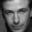
\includegraphics[width=.35\linewidth]{cropped/baldwin0.jpg}
  \caption{baldwin0.jpg}
  \label{fig:sfig1}
\end{subfigure}
\begin{subfigure}{.35\textwidth}
 \centering
  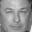
\includegraphics[width=.35\linewidth]{cropped/baldwin1.jpg}
  \caption{baldwin1.jpg}
  \label{fig:sfig2}
\end{subfigure}%
\begin{subfigure}{.35\textwidth}
 \centering
  
\includegraphics[width=.35\linewidth]{cropped/baldwin2.jpg}
  \caption{baldwin2.jpg}
  \label{fig:sfig3}
\end{subfigure}
\begin{subfigure}{.35\textwidth}
 \centering
  
\includegraphics[width=.35\linewidth]{cropped/baldwin3.jpg}
  \caption{baldwin3.jpg}
  \label{fig:sfig4}
\end{subfigure}%
\begin{subfigure}{.35\textwidth}
 \centering
  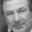
\includegraphics[width=.35\linewidth]{cropped/baldwin4.jpg}
  \caption{baldwin4.jpg}
  \label{fig:sfig5}
\end{subfigure}
\begin{subfigure}{.35\textwidth}
 \centering
  
\includegraphics[width=.35\linewidth]{cropped/harmon50.jpg}
  \caption{harmon50.jpg}
  \label{fig:sfig6}%
\end{subfigure}
\caption{Example cropped figures from dataset}
\label{fig:pics}
\end{figure*}

\begin{figure*}[!ht]
\begin{subfigure}{.35\textwidth}
 \centering
  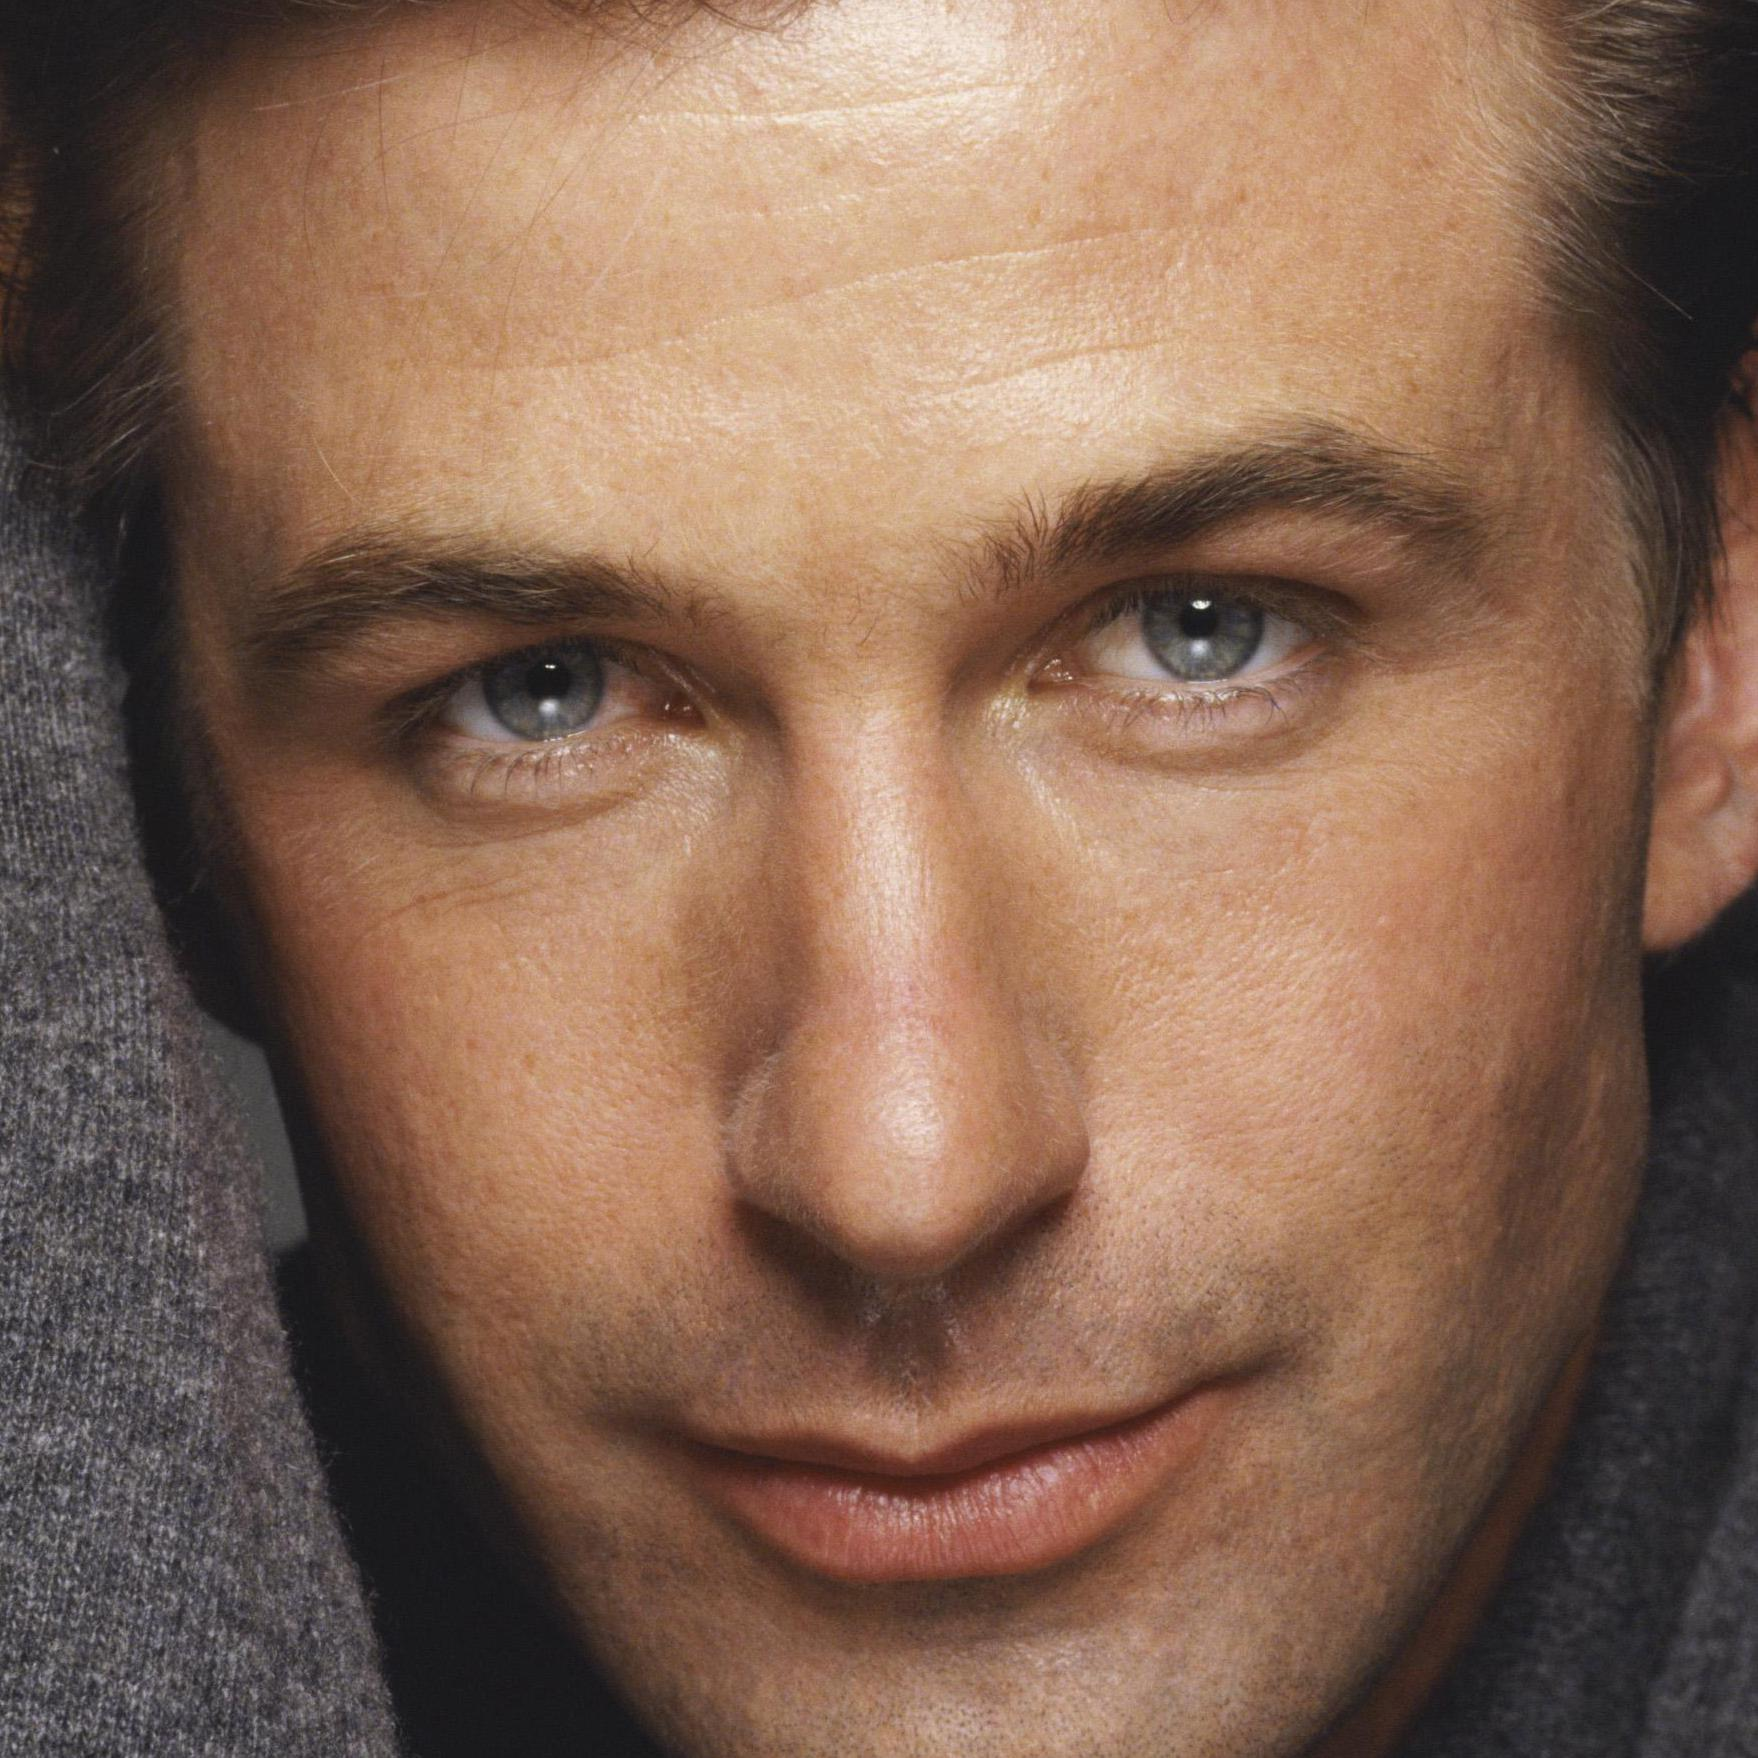
\includegraphics[width=.35\linewidth]{uncropped/baldwin0.jpg}
  \caption{baldwin0.jpg}
  \label{fig:sfig1}
\end{subfigure}
\begin{subfigure}{.35\textwidth}
 \centering
  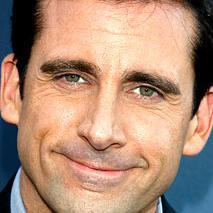
\includegraphics[width=.35\linewidth]{uncropped/carell39.jpg}
  \caption{carell39.jpg}
  \label{fig:sfig2}
\end{subfigure}%
\begin{subfigure}{.35\textwidth}
 \centering
  
\includegraphics[width=.35\linewidth]{uncropped/harmon50.jpg}
  \caption{harmon50.jpg}
  \label{fig:sfig3}
\end{subfigure}
\caption{Example uncropped figures from dataset}
\label{fig:pics}
\end{figure*}

\end{homeworkProblem}
\clearpage
%----------------------------------------------------------------------------------------
%	PROBLEM 2
%----------------------------------------------------------------------------------------

\begin{homeworkProblem}
\noindent \textit{Seperate Dataset into Training Set, Validation Set and Test Set}

The seperation of the dataset is done using the seperate\_sets function in faces.py. The input of the function is the path of the directory where the cropped images are saved. The function would create a folder named ``sets'' in the current directory and three sub folders in the ``sets'' folder. The images will be readed as a list and shuffled. The first ten occurrences of each character in the shuffled list will be copied to the test\_set folder, the next ten will be copied to the validation\_set folder. The next seventy will be copied to the training\_set folder. Notice that there is only 88 pictures of Gilpin, so there is only 68 of her photo in the training set.


\end{homeworkProblem}
\clearpage

%----------------------------------------------------------------------------------------
%	PROBLEM 3
%----------------------------------------------------------------------------------------

\begin{homeworkProblem}
\noindent \textit{Use Linear Regression to build a classifier of two Actors' photoes}

For this question, I choose to minimized the quadratic cost function $\sum_{i = 1}^{m} (\theta^{T}X^{i} - y^{i})^{2})$. The value of the cost function on the training set is 0.26931154634136567. The performance on the training set is 100\% correctness.The value of the cost function on the validation set is 1.3211391164441706. The performance on the validation set is 95\% correctness. 

In order to get the system to work, the alpha value is at most 0.00002, a value greater than that would make the value of the cost function keep growing and eventually overflow. It is possibly becuase the large alpha make the theta move too much. If the theta is too small, it will need more iterations to reach a similar value of the cost function.

The tester\_p3 load each image from the desired set and it use the classifier\_p3 to find out who that person is and compare it to the correct answer. At the end, the function would print the correct rate and the cost function for that set.

\begin{lstlisting}[language=python]
def classifier_p3(x, theta):
    x = np.hstack((np.ones(1), x))
    h_x = np.dot(theta.T, x)
    if h_x > 0.5:
        return actors[3]
    else:
        return actors[5]

def tester_p3(directory, theta):
    images = os.listdir(directory)
    correct = 0.0
    total = 0.0
    x_temp = []
    y_temp = []
    for image in images:
        cur_name = re.search('[a-z]+', image).group(0)
        flag = -1
        if cur_name == actors[3]:
            flag = 1
        elif cur_name == actors[5]:
            flag = 0

        if flag != -1:
            im = imread(directory+"/"+image)
            im = im.reshape(1024)
            im = im.astype(float)
            im = im/255
            x_temp.append(im)
            y_temp.append(flag)
            total += 1
            result = classifier_p3(im, theta)
            if result == cur_name:
                correct += 1

    y_temp = np.array(y_temp)
    x_temp = np.array(x_temp)
    x_temp = np.vstack((np.ones((1, x_temp.T.shape[1])), x_temp.T))
    cost = f_p3(x_temp,y_temp,theta)
    print directory + ' tested'
    print "Cost function's value is " + str(cost)
    print str(correct) + "/" + str(total) + " is correct. The accuracy rate is " + str(correct/total*100) + "%."
\end{lstlisting}
\end{homeworkProblem}
\clearpage
%----------------------------------------------------------------------------------------
%	PROBLEM 4
%----------------------------------------------------------------------------------------

\begin{homeworkProblem}
\noindent \textit{Showing Thetas As Heatmap}
\vskip 0.2in
Part A)\newline
The left figure is the theta obtained from P3, the right figure is the theta from training using a training set that contains only two images of each actor.
The left one doesn't looks like a face because while training in P3, the value of the cost function gets to pretty small so the theta is overfitted to the training set.
\vskip 0.2in
Part B)\newline
To make theta contains a face, I stop the gradient descent fairly early at 1000 iteration when the cost function is still around 7. And for my own interest, I tested the performance of this theta on the training set is about 97\%, while on the validation set, its performance is 100\%
\vskip 0.2in
\begin{figure*}[!ht]
\begin{subfigure}{.5\textwidth}
 \centering
  
\includegraphics[width=.5\linewidth]{p4_1.JPG}
  \caption{Full set}
  \label{fig:sfig1}
\end{subfigure}
\begin{subfigure}{.5\textwidth}
 \centering
  \includegraphics[width=.5\linewidth]{P4_2.JPG}
  \caption{Two each}
  \label{fig:sfig2}
\end{subfigure}%
\caption{Part4 (a)}
\label{fig:p4a}
\end{figure*}

\begin{figure*}[!ht]
 \centering
    \includegraphics[scale=4]{P4_3.JPG}
    \caption{Part4 (b)}
    \label{fig:p4b}
\end{figure*}


\end{homeworkProblem}
\clearpage

%----------------------------------------------------------------------------------------
%	PROBLEM 5
%----------------------------------------------------------------------------------------

\begin{homeworkProblem}
\noindent \textit{Demonstration of overfit}

Below is the plotting for performance of the classifiers on the training and validation sets vs the size of the training set. To demonstrate the overfitting, I run gradient descent with training sets with various numbers of photoes of the 6 actors in act for 100000 iteration. Then use all the photoes of actors not in act as the validation set. First when the training set increase from 100 to 400, we can see a increase in the performance on the validation set. Because as the size of training set gets bigger, it is harder for the model to overfit those irregularities because the only contribute to a smaller and smaller percentage of the data. However, we can see that when the size of the training set increase from 400 to 500, the performance on the training set stays 100, while the performance on the test set drops slightly,  this could be some spurious regularities in the training set builds up enough to affect the calculation of $\theta$.

\begin{figure*}[!ht]
 \centering
    \includegraphics[scale=0.8]{P5.JPG}
    \caption{Demonstration of Overfitting}
    \label{fig:p5}
\end{figure*}

\end{homeworkProblem}
\clearpage
%----------------------------------------------------------------------------------------
%	PROBLEM 6
%----------------------------------------------------------------------------------------

\begin{homeworkProblem}
\noindent \textit{Multi-classification problem}

Part A)\newline
\begin{figure*}[ht]
 \centering
    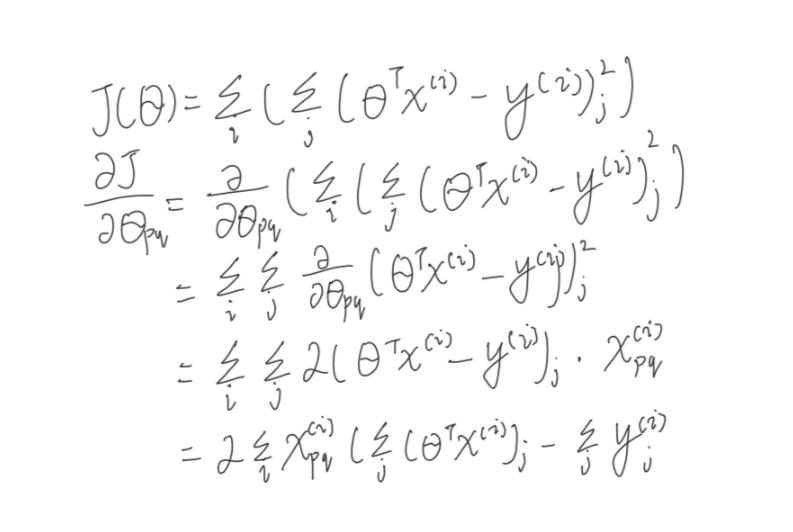
\includegraphics[scale=0.8]{p6.png}
    \caption{Derivative}
    \label{fig:p5}
\end{figure*}
\vskip 0.2in
Part B)\newline
$\frac{\partial J}{\partial \theta} = \left(\begin{bmatrix} \frac{\partial J}{\partial \theta_{11}} \ldots \frac{\partial J}{\partial \theta_{1k}} \\ \vdots \\ \frac{\partial J}{\partial \theta_{n1}} \ldots \frac{\partial J}{\partial \theta_{nk}} \end{bmatrix} \right)$\newline
Each value in $\frac{\partial J}{\partial \theta}$ correspond to one such $\frac{\partial J}{\partial \theta_{pq}}$ solved in 6(a). Each value in$(\theta^{T}X - Y)$ correspond to the $(\theta^{T}X^{i}-y^{i})_j $ for some i, j. Transpose the whole part and dot product it by $2X$. Each entry in $2X(\theta^{T}X - Y)^{T}$ correspond to $2X_{pq}^{i} (\theta^{T}X^{i}- y^{i})_j$ value for one of the k columns of the theta with one of the n sample images. 
Define k as the number of labels, m as the number of training example, n as the number of pixels in one example plus 1:\newline
The dimension of  $\theta$ is $n * k$\newline
The dimension of $X $ is $n * m$\newline
The dimension of $Y$ is $k * m$\newline
\vskip 0.2in
Part C)\newline
The f\_p6 below is the cost function, df\_p6 below is the gradient function. I have already transposed X and add a row of 1s before passing it to the function to avoid repeating the process during the gradient descent.
\begin{lstlisting}[language=python]
def f_p6(x, y, theta):
    return np.sum((np.dot(theta.T, x)- y) ** 2)

def df_p6(x, y, theta):
    return 2 * (np.dot(x, (np.dot(theta.T, x)- y).T))
\end{lstlisting}
\clearpage
Part D)\newline
The following code generates a random x with size 5x10, a random y with size 3x10 and a random theta with size 5x3. Then calculate and print the gradient on five directions. And in the end calculate and print the gradient using df\_p6. We can check whether the values are close to the result. The result are shown below. It is easy to see that the results are almost identical.I choose a small enough h too demonstrate that when h gets to really small, the result from the two methods is almost identical
\begin{lstlisting}[language=python]

def part_6():
    np.random.seed(0)
    x = np.random.rand(5,10)
    y = np.random.rand(3,10)
    theta = np.random.rand(5,3)
    h = 0.0000001
    h_array = np.zeros((5,3))
    for i in range(5):
        h_array[i][1] = h
        print 'changing theta at [' + str(i)+', ' +  '1]'
        print (f_p6(x, y, theta+np.array(h_array)) - f_p6(x, y, theta-np.array(h_array)))/(2*h)
        h_array[i][1] = 0.0
    print df_p6(x, y, theta)
    
Doing part6
changing theta at [0, 1]
9.38697874986
changing theta at [1, 1]
9.87473635305
changing theta at [2, 1]
10.1618410397
changing theta at [3, 1]
8.29621136234
changing theta at [4, 1]
5.53991927887
[[ 14.009767     9.38697875   7.73695701]
 [ 14.29292737   9.87473635   7.21595527]
 [ 14.41686725  10.16184104   7.59067318]
 [ 13.31166437   8.29621136   8.07369466]
 [  6.73157401   5.53991927   3.35461769]]


\end{lstlisting}

\end{homeworkProblem}
\clearpage
%----------------------------------------------------------------------------------------
%	PROBLEM 7
%----------------------------------------------------------------------------------------

\begin{homeworkProblem}
\noindent \textit{Implement Multi-classification}
The performance on the validation set is 95.6937799043\%. The performance on the validation set is 95.6937799043\%. I choose to use 0.000001 as alpha because that is the greatest alpha that would not induce an overflow when calculating the gradient. I stop the gradient descent early at 20000 iteration to avoid overfitting. Stopping it earlier would make the performance on validation set decrease. The output of the model will be a array of 6 number representing the probabilities of this images being each person. Find out the index of the max of the array and who that index respects to.  For example, if output is [0.01, 0.03, 0.23, 0.85, 0.32, 0.05] and y for Baldwin is [0,0,0,1,0,0], then we say this is a picture of Baldwin.



\end{homeworkProblem}
\clearpage
%----------------------------------------------------------------------------------------
%	PROBLEM 8
%----------------------------------------------------------------------------------------

\begin{homeworkProblem}
\noindent \textit{Images of thetas for Multi-classification}
Below are the 6 images for the theta

\begin{figure*}[!ht]
\begin{subfigure}{.35\textwidth}
 \centering
  
\includegraphics[width=.35\linewidth]{p8_0.jpg}
  \caption{bracco}
  \label{fig:sfig1}
\end{subfigure}
\begin{subfigure}{.35\textwidth}
 \centering
  
\includegraphics[width=.35\linewidth]{p8_1.jpg}
  \caption{gilpin}
  \label{fig:sfig2}
\end{subfigure}%
\begin{subfigure}{.35\textwidth}
 \centering
  
\includegraphics[width=.35\linewidth]{p8_2.jpg}
  \caption{harmon}
  \label{fig:sfig3}
\end{subfigure}
\begin{subfigure}{.35\textwidth}
 \centering
  
\includegraphics[width=.35\linewidth]{p8_3.jpg}
  \caption{baldwin}
  \label{fig:sfig4}
\end{subfigure}%
\begin{subfigure}{.35\textwidth}
 \centering
  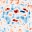
\includegraphics[width=.35\linewidth]{p8_4.jpg}
  \caption{hader}
  \label{fig:sfig5}
\end{subfigure}
\begin{subfigure}{.35\textwidth}
 \centering
  
\includegraphics[width=.35\linewidth]{p8_5.jpg}
  \caption{carell}
  \label{fig:sfig6}%
\end{subfigure}
\caption{Images of theta}
\label{fig:pics}
\end{figure*}

\end{homeworkProblem}
\clearpage
%----------------------------------------------------------------------------------------

\end{document}
